\documentclass[12pt,a4paper]{report}

%====================== PACKAGES ======================

\usepackage[english]{babel}
\usepackage[utf8x]{inputenc}
%pour gérer les positionnement d'images
\usepackage{float}
\usepackage{amsmath}
\usepackage{graphicx}
\usepackage[colorinlistoftodos]{todonotes}
\usepackage{url}
%pour les informations sur un document compilé en PDF et les liens externes / internes
\usepackage{hyperref}
%pour la mise en page des tableaux
\usepackage{array}
\usepackage{tabularx}
%espacement entre les lignes
\usepackage{setspace}
\usepackage{parskip}
%modifier la mise en page de l'abstract
\usepackage{abstract}
%police et mise en page (marges) du document
\usepackage[T1]{fontenc}
\usepackage{times}
\usepackage[top=2cm, bottom=2cm, left=2.5cm, right=2.5cm]{geometry}
%Pour les galerie d'images
\usepackage{subfig}
%pour les graphes
\usepackage{tikz}
\usetikzlibrary{arrows.meta}

%====================== INFORMATION ET REGLES ======================

% Configuration de l'espacement
\onehalfspacing

% Configuration des légendes de figures
\captionsetup{font={small,rm},labelsep=period,skip=4pt}

\hypersetup{							% Information sur le document
pdfauthor = {Florence PAUTET},			% Auteurs
pdftitle = {Nom du Projet -
			Sujet du Projet},			% Titre du document
pdfsubject = {Rapport de stage},		% Sujet
pdfkeywords = {Tag1, Tag2, Tag3},	% Mots-clefs
pdfstartview={FitH}}					% ajuste la page à la largueur de l'écran

%======================== DEBUT DU DOCUMENT ========================

\begin{document}

% parameters tiks
\tikzset{every node/.style={circle, draw, minimum size=1.2cm, text width=1.2cm, align=center, font=\small}}
\tikzset{>={Stealth[scale=2]}}

%ligne horizontale
\newcommand{\HRule}{\rule{\linewidth}{0.5mm}}
%espacement entre les lignes d'un tableau
\renewcommand{\arraystretch}{1.5}

%page de garde
\begin{titlepage}

% Logos en haut de page
\begin{center}
\begin{figure}[htbp]
\centering
\begin{minipage}{0.45\textwidth}
\centering

\includegraphics[width=0.9\textwidth]{./logos/logo_sorbonne.png}
\end{minipage}%
\hfill
\begin{minipage}{0.45\textwidth}
\centering

\includegraphics[width=0.9\textwidth]{./logos/Logo_Institut_Pasteur.png}
\end{minipage}
\end{figure}

\vspace{1.5cm}

% Titre du rapport
\HRule \\[0.6cm]
{\huge \bfseries \textsc{Nom du Projet}}\\[0.4cm]
{\Large \textit{Sujet du Projet}}\\[0.4cm]
\HRule \\[1.5cm]

% Informations académiques
\large
\textbf{Master 2 Internship Report}\\[0.3cm]
Specialisation: Bioinformatics and Modelisation\\
\textit{Academic year 2024--2025}

\vspace{1.5cm}

% Informations personnelles
\fbox{\begin{minipage}{0.8\textwidth}
\vspace{0.5cm}
\begin{tabular}{l @{\hskip 1cm} l}
\textbf{Intern:} & Florence \textsc{Pautet} \\[0.3cm]
\textbf{Supervisor:} & Yoann \textsc{Dufresne} \\[0.3cm]
\textbf{Institution:} & Sorbonne University\\[0.3cm]
\textbf{Host Organization:} & Pasteur Institut \\[0.3cm]
\textbf{Internship Period:} & From February 10 to July 31, 2025 \\[0.3cm]
\end{tabular}
\vspace{0.5cm}
\end{minipage}}

\vfill

% Pied de page optionnel
\today\\
% \textit{\small Ce rapport est présenté dans le cadre de l'obtention du diplôme de Master 2 de la Sorbonne Université}

\end{center}
\end{titlepage}

\newpage
\input{./parts/abstract.tex}

\tableofcontents
\thispagestyle{empty}



%====================== INCLUSION DES PARTIES ======================

\newpage
\setcounter{page}{1}

\chapter{Présentation du projet}

Intro\footnotemark\\
%note en bas de page

\section{Graphe de de Bruijn}


%Contenu de la note précédemment marquée avec \footnotemark
\footnotetext{Note bas de page "intro"}
Bla(cf. ref. \cite{cite6}).

\chapter{Preliminaries}

\section{De Bruijn Graphs}

\subsection{Definition}

A \textbf{kmer} is a string of length $k$ over the alphabet $\Sigma$.

For $R$ a given set of strings over $\Sigma$, the representing \textbf{de Bruijn graph} of order $k$ is the directed graph $G = (V, E)$ where:
\begin{itemize}
    \item Each vertex corresponds to a unique kmer in $R$.
    \item There is a directed edge from vertex $u$ to vertex $v$ if and only if the suffix of $u$ of length $k-1$ is identical to the prefix of $v$ of length $k-1$
\end{itemize}

In genomic applications, the alphabet $\Sigma$ typically consists of the four nucleotides: $\Sigma = \{A, C, G, T\}$.

\begin{tikzpicture}[scale=1.5]
    % First row of nodes
    \node (A1) at (3, 2) {AGC};
    
    % Second row of nodes
    \node (B1) at (0, 0) {GCT};
    \node (B2) at (2, 0) {CTG};
    \node (B3) at (4, 0) {TGA};
    \node (B4) at (6, 0) {GAG};
    \node (B5) at (8, 0) {AGT};
    
    % Third row of nodes
    \node (C2) at (2, -2) {CTA};
    \node (C3) at (4, -2) {TAA};
    \node (C4) at (6, -2) {AAG};
    
    % Edges between nodes
    \draw[->] (B1) -- (B2);
    \draw[->] (B2) -- (B3);
    \draw[->] (B3) -- (B4);
    \draw[->] (B4) -- (B5);

    \draw[->] (B1) -- (C2);
    \draw[->] (C2) -- (C3);
    \draw[->] (C3) -- (C4);
    \draw[->] (C4) -- (B5);

    
    \draw[<-] (B1) -- (A1);
    \draw[<-] (A1) -- (B4);
  \end{tikzpicture}

\subsection{Compact de Bruijn Graphs}

\begin{tikzpicture}[scale=1.5]
    % First row of nodes
    \node (A1) at (2, 2) {AGC};
    
    % Second row of nodes
    \node (B1) at (0, 0) {GCT};
    \node (B2) at (2, 0) {CTGA};
    \node (B3) at (4, 0) {GAG};
    \node (B4) at (6, 0) {AGT};
    
    % Third row of nodes
    \node (C1) at (3, -2) {CTAAG};
    
    % Edges between nodes
    \draw[->] (B1) -- (B2);
    \draw[->] (B2) -- (B3);
    \draw[->] (B3) -- (B4);

    \draw[->] (B1) -- (C1);
    \draw[->] (C1) -- (B4);

    
    \draw[<-] (B1) -- (A1);
    \draw[<-] (A1) -- (B3);
  \end{tikzpicture}

\subsection{Colored de Bruijn Graphs}

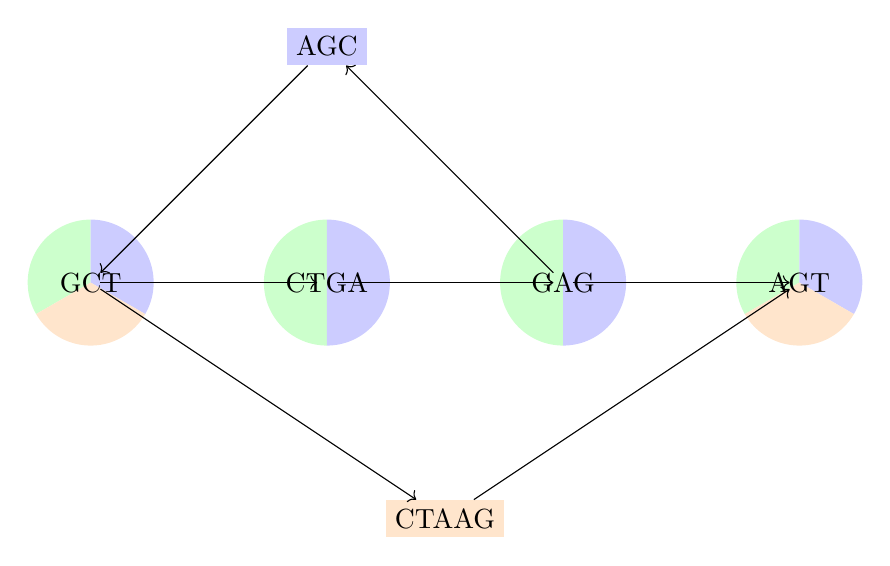
\begin{tikzpicture}[scale=1.5]
    % Define the size of the pic circles (note: pic and nodes are not the same)
    \def\a{1.6}
    % Style definitions for each row
    \tikzset{
        % one color
        one color/.style={fill=#1},
        % two colors
        pics/two colors/.style args=
        {#1|#2|label=#3}{code={%
            \fill[#1] (0,\a/2) arc(90:270:\a/2)--cycle;
            \fill[#2] (0,\a/2) arc(90:-90:\a/2)--cycle;
            \path (0,0) node[label={center:#3}] () {};
        }},
        % three colors
        pics/three colors/.style args=
        {#1|#2|#3|label=#4}{code={%
            \fill[#1] (0,\a/2) arc(90:210:\a/2)--(0,0)--cycle;
            \fill[#2] (0,\a/2) arc(90:-30:\a/2)--(0,0)--cycle;
            \fill[#3] (210:\a/2) arc(210:330:\a/2)--(0,0)--cycle;
            \path (0,0) node[label={center:#4}] () {};
        }}
    }
    % First row of nodes
    \node[one color=blue!20] (A1) at (2, 2) {AGC};

    % Second row of nodes
    \pic (B1) at (0, 0) {three colors={green!20|blue!20|orange!20|label=GCT}};
    \pic (B2) at (2, 0) {two colors={green!20|blue!20|label=CTGA}};
    \pic (B3) at (4, 0) {two colors={green!20|blue!20|label=GAG}};
    \pic (B4) at (6, 0) {three colors={green!20|blue!20|orange!20|label=AGT}};

    % Third row of nodes
    \node[one color=orange!20] (C1) at (3, -2) {CTAAG};

    % Edges between nodes
    \draw[->] (B1) -- (B2);
    \draw[->] (B2) -- (B3);
    \draw[->] (B3) -- (B4);

    \draw[->] (B1) -- (C1);
    \draw[->] (C1) -- (B4);

    \draw[<-] (B1) -- (A1);
    \draw[<-] (A1) -- (B3);
\end{tikzpicture}


% \begin{figure}[htbp]
%     \centering
%     % Placeholder for a de Bruijn graph illustration
%     % \includegraphics[width=0.8\textwidth]{debruijn_graph_example.png}
%     \caption{Example of a de Bruijn graph constructed from short reads. (a) Original reads. (b) Extraction of $k$-mers ($k=3$). (c) Resulting de Bruijn graph where nodes are $(k-1)$-mers and edges represent $k$-mers. (d) A possible Eulerian path through the graph (highlighted) representing a candidate assembly.}
%     \label{fig:debruijn}
% \end{figure}

\input{./parts/results.tex}

\input{./parts/conclusion.tex}

%Ne pas numéroter cette partie
\part*{Annexes}
%Rajouter la ligne "Annexes" dans le sommaire
\addcontentsline{toc}{part}{Annexes}


\chapter*{Annexe 1}
\addcontentsline{toc}{chapter}{Annexe 1}

%changer le format des sections, subsections pour apparaittre sans le num de chapitre
\makeatletter
\renewcommand{\thesection}{\@arabic\c@section}
\makeatother

%recommencer la numérotation des section à "1"
\setcounter{section}{0}
Intro
\section{Partie 1}
Bla
\subsection{Sous-partie 1}
Bla
\subsection{Sous-partie 2}
Bla
\section{Partie 2}
Bla
\subsection{Sous-partie 1}
Bla

\chapter*{Annexe 2}
\addcontentsline{toc}{chapter}{Annexe 2}

%recommencer la numérotation des section à "1"
\setcounter{section}{0}
\begin{itemize}
\item item1;
\item item2;
\item item3;
\item item4.
\end{itemize}

Bla

\begin{center}
\textsc{Attention !}

\textit{Texte d'avertissement}
\end{center}

Bla

\newpage

\section{Partie 3}
Bla
% \begin{figure}[!ht]
% \begin{center}
% \includegraphics[height=8cm]{presentation/schema}
% \end{center}
% \caption[schema]{Presentation schema}
% \end{figure}

\paragraph*{Paragraphe 1}
~\\
\hskip7mm
Bla
\paragraph*{Paragraphe 2}
~\\
\hskip7mm
Bla

%tableau centré à taille variable qui s'ajuste automatiquement suivant la longueur du contenu
\begin{figure}[!h]
    \begin{center}
    \begin{tabular}{|l|l|l|l|l|}
      \hline
      Solution & Critère 1 & Critère 2 & Critère 3 & Critère 4\\
      \hline
      Solution 1(cf. ref. \cite{cite0}) & Oui & Oui & Oui & Oui \\
      Solution 2(cf. ref. \cite{cite1}) & Oui & Oui & Oui & Non \\
      Solution 3(cf. ref. \cite{cite2}) & Oui (sauf telle chose) & Non & Non & Oui\\
      Solution 4(cf. ref. \cite{cite3}) & Oui& Non & Oui & Non\\
      Solution 5(cf. ref. \cite{cite4}) & Oui (uniquement ceux-ci) & Non & Oui & Non\\
      \hline
    \end{tabular}
    \end{center}
    \caption{Tableau récapitulatif des solutions}
\end{figure}


%galerie d'image
% \begin{figure}[htp]
%     \centering
%     \subfloat[Première image]{\label{fig:première}\includegraphics[scale=0.8]{resultats/gallerie}}
%     ~ %espace entre deux images sur une même ligne
%     \subfloat[Deuxième image]{\label{fig:deuxième}\includegraphics[scale=0.8]{resultats/gallerie}}
%     ~
%     \subfloat[Troisième image]{\label{fig:troisième}\includegraphics[scale=0.8]{resultats/gallerie}}
%     ~\\ %saute une ligne dans la galerie d'image
%     \subfloat[Quatrième image]{\label{fig:quatrième}\includegraphics[scale=0.8]{resultats/gallerie}}
%     ~
%     \subfloat[Cinquième image]{\label{fig:cinquième}\includegraphics[scale=0.8]{resultats/gallerie}}
%     \caption{Différents screenshots quelque chose, en gallerie}
%     \label{fig:gallerie1}
% \end{figure}

\newpage

%récupérer les citation avec "/footnotemark"
\nocite{*}

%choix du style de la biblio
\bibliographystyle{plain}
%inclusion de la biblio
\bibliography{bibliographie.bib}

\end{document}